\cite{AIShackCannyEdge} 

Considered the ultimate edge detector. Clean, thing edges that are well connected to nearby edges. 

Multistage edge detector:

\begin{enumerate}
\item Preprocessing
\item Calculating Gradients
\item Nonmaximum suppression
\item Thresholding with hysterysis.
\end{enumerate}

Two key parameters given are upper and lower thresholds; upper is used to mark definite edges, lower is used for faint pixels that are part of an edge.

\subsection{Preprocessing}
Edge detectors prone to noise, gaussian blur filter helps. Typically need to perform this step yourself even with software packages. Typically, 5x5 Gaussian filter with standard deviation of 1.4 is used.

\subsection{Calculating Gradients}

Gradient is calculated at every point in image. Magnitude of gradient at point determines if it lies on an edge or not. Higher the gradient the greater the likelihood of an edge. Direction of gradient shows how image is oriented. The standard \emph{Sobel Edge Detector} is used. Magnitude of the gradient is:

\begin{equation}
m = \sqrt{G_x^2 + G_y^2}
\end{equation}

And the direction is:

\begin{equation}
\theta = arctan(\frac{G_y}{G_x})
\end{equation}

Where $G_x$ and $G_y$ are the derivatives for the given point. The gradients are calculated by using a convolution kernels which approximate the derivative in the X and Y directions.

\subsection{Non maximum suppression}
Check edges in four directions: Vertical, Horizontal, and the two diagonals. For each case, the middle pixel is checked against neighboring pixels to see if it is a maximum and is suppressed if it is not.

\begin{figure}[ht!]
{
\centering

\includegraphics[width=0.5\textwidth]{eps_pics/possible-neighbors}
\caption{Possible directions of an edge}
\label{fig:possibleNeighbors}
}
\end{figure}

\subsubsection{Gradient from 22.5 to 67.5}

This case means that the edge goes from the top right to the bottom left. To check if an edge exists for this case, first need to check if gradient is maximum at this point. To do this, compare gradient magnitude of middle pixel to that of the top left and lower right pixels. If it's a maximum and its magnitude is greater than threshold than its an edge.

\begin{figure}[ht!]
{
\centering
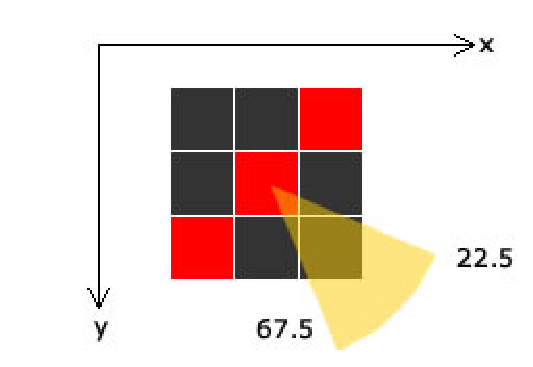
\includegraphics[width=0.5\textwidth]{eps_pics/edge-direction-451}
\caption{Diagonal south to north case}
\label{fig:edge_direction_south_to_north}
}
\end{figure}


\begin{figure}[ht!]
{
\centering
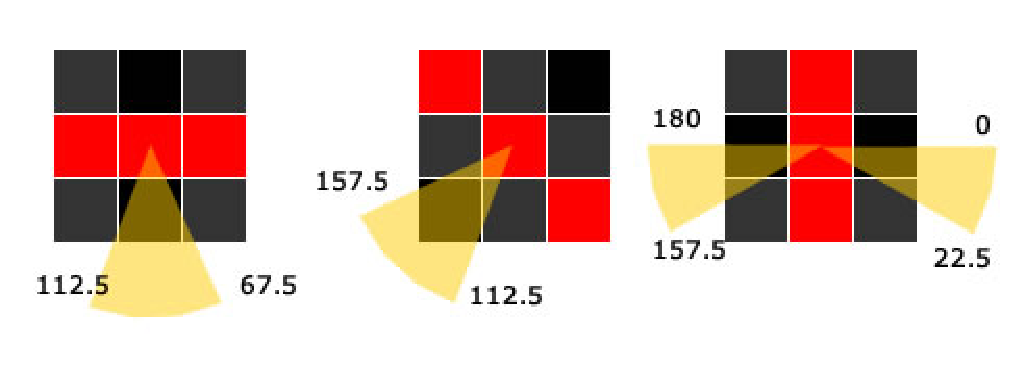
\includegraphics[width=0.5\textwidth]{eps_pics/edge-direction-all}
\caption{Remaining 3 edge cases}
\label{fig:edge_direction_all}
}
\end{figure}
